\documentclass{article}
\usepackage[utf8]{inputenc}
\usepackage{amsmath}
\usepackage{mathtools}
\usepackage[numbered, framed]{matlab-prettifier}

\begin{filecontents*}{task2c_code.m}
    syms x(t);
    
    egn = diff(x, t, 2) - 5*x == diff(x, t, 1) + t + 2*x + 3;
    Dx = diff(x,t, 1);
    cond = [Dx(0) == 4, x(0) == 3];
    
    xSolt(t) = dsolve(egn, cond);
    
    t = linspace(0, 1);
    
    figure
    plot(t, xSolt(t));

\end{filecontents*}

\begin{filecontents*}{task2d_code.m}
    syms p t X;
    f = t + 3;
    F = laplace(f, t, p);
    X1 = p * X - 3;
    X2 = p * X1 - 4;
    S = solve(X2 - X1 - 7*X == F, X);
    s = ilaplace(S, p, t);

\end{filecontents*}

\lstset{
  style = Matlab-editor,
  basicstyle = \mlttfamily,
  escapechar = ",
  mlshowsectionrules = true,
}

\title{Control Theory Homework 1}
\author{Kamil Kamaliev, Var q}
\date{February 2020}

\begin{document}
    \maketitle
    
    \paragraph{2.A}
        
        $$x^{\prime\prime}-5x=x^\prime + t + 2x + 3, x^{\prime}(0)=4, x(0) = 3$$ 
        $$x^{\prime\prime} = x^\prime + t + 7x + 3$$
        
        
        Simulink schema:
        
       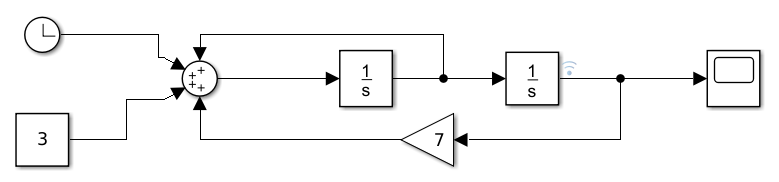
\includegraphics[scale=0.5]{task2a_schema.png}
       
       \vskip
        
       Plot:
       
       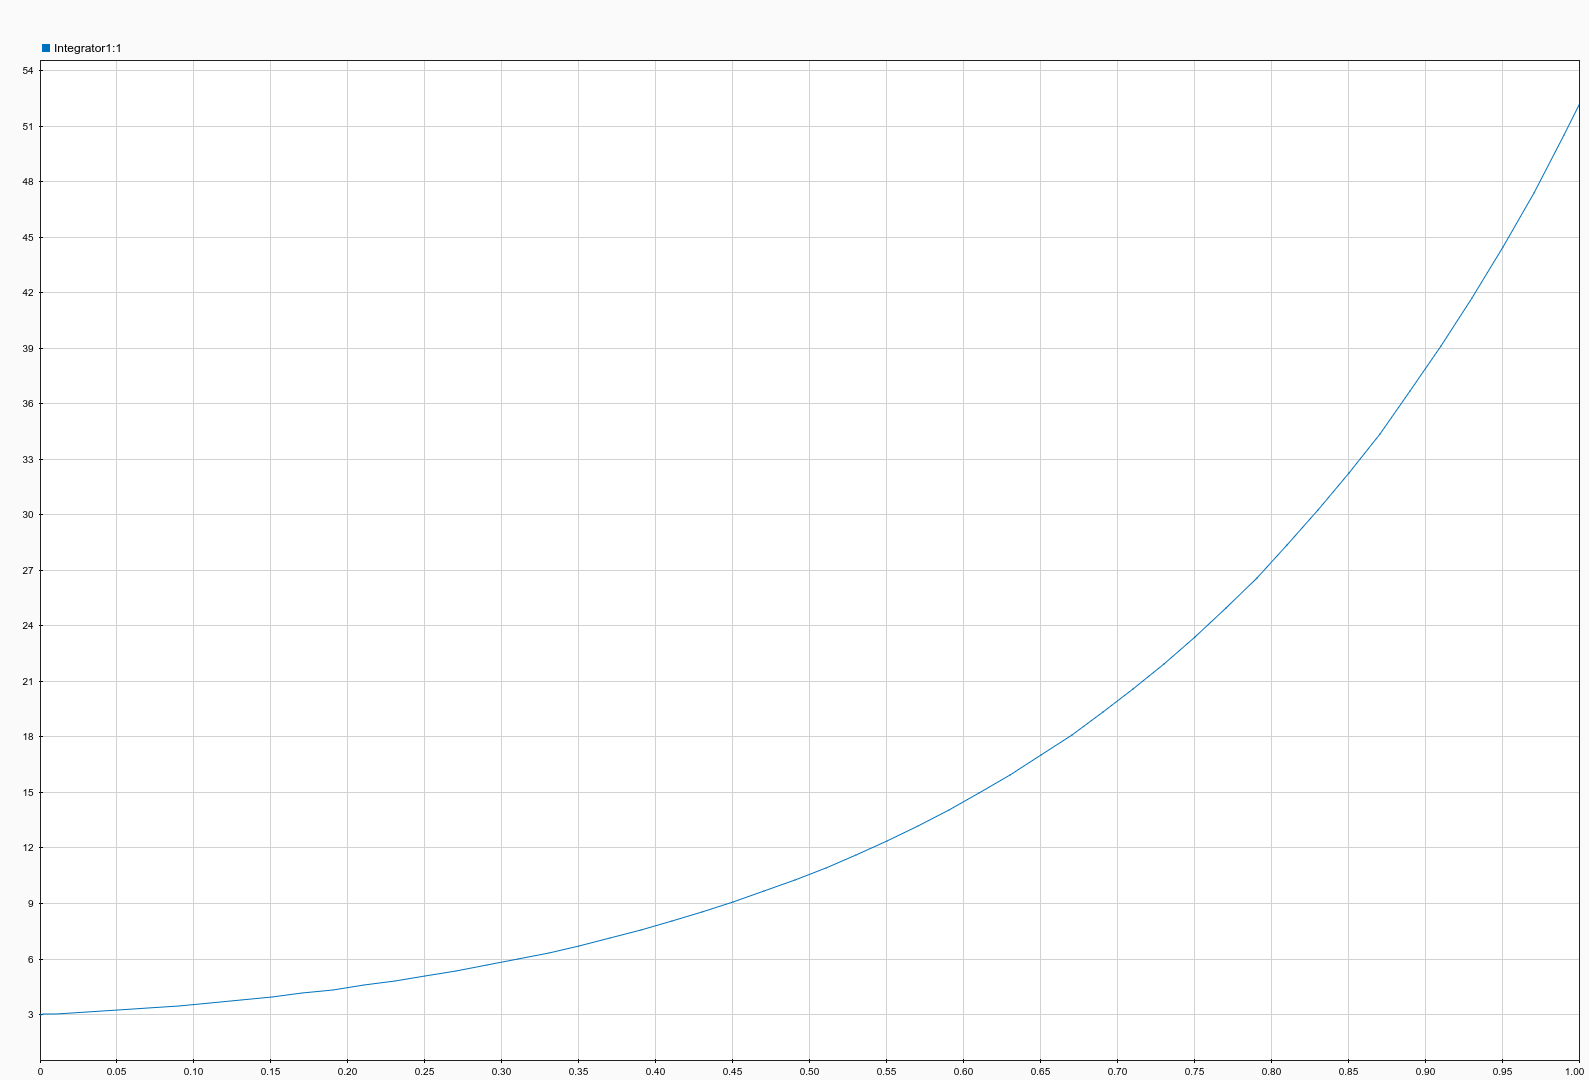
\includegraphics[scale=0.3]{task2a_plot.png}
        
    \newpage
    
    \paragraph{2.B}
        
        Calculations of TF:
        
        $$x^{\prime\prime} = x^\prime + t + 7x + 3$$
        $$x^{\prime\prime} - x^\prime - 7x = t + 3$$
    
    Substitute $u(t) = t + 3$ and apply Laplace transform to both sides.
    
        $$LT(x^{\prime\prime} - x^\prime - 7x) = LT(u(t))$$
        $$X(p)(p^2 - p - 7) = U(p)$$
        $$\frac{X(p)}{U(p)} = \frac{1}{p^2 - p - 7}$$
        
        Simulink schema:
        
       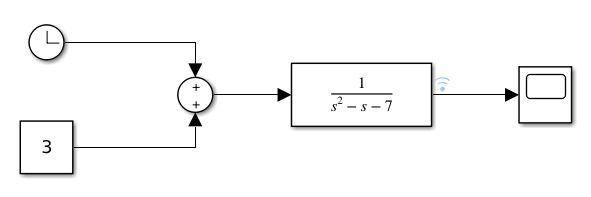
\includegraphics[scale=0.5]{task2b_schema.png}
       
       \vskip
        
       Plot:
       
       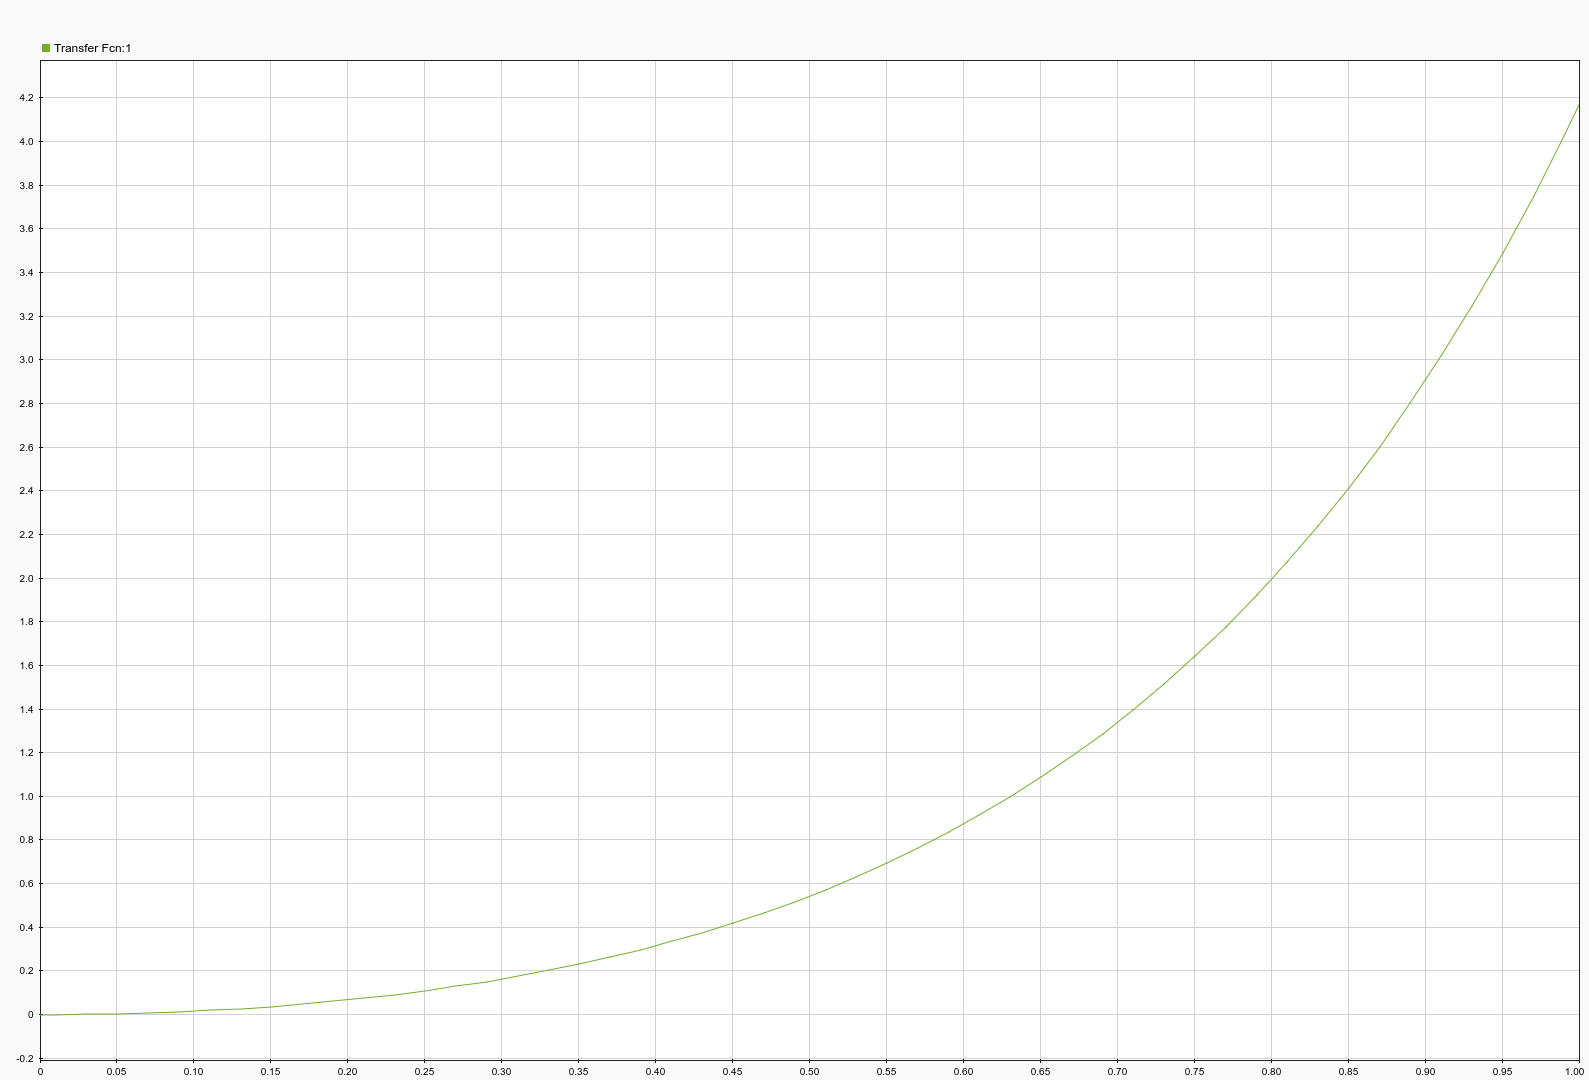
\includegraphics[scale=0.3]{task2b_plot.png}
    
    \newpage
    
     \paragraph{2.C}
     
        Plot:
       
       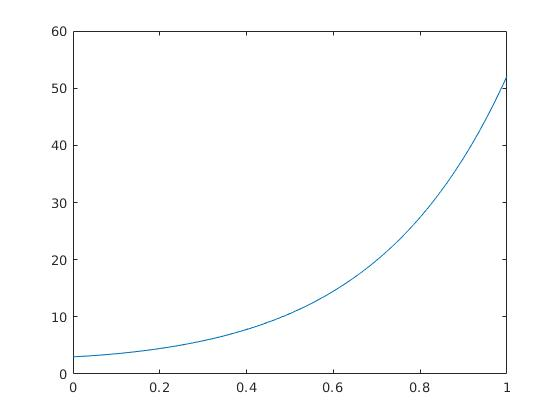
\includegraphics[scale=0.5]{task2c_plot.jpg}
        
        \lstinputlisting[caption={MATLAB code}]{task2c_code.m}
    
    \newpage
    
     \paragraph{2.D}
     
    Code:
     \lstinputlisting[caption={MATLAB code}]{task2d_code.m}
     
     
     \paragraph{3}
     
     $$3x^{\prime\prime} + 3x^{\prime} - 3 = 2t - 2, y = 3x^{\prime}$$
     $$x^{\prime\prime} + x^{\prime} - 1 = \frac{2t - 2}{3}$$
     $$x^{\prime\prime} = \frac{2t}{3} - x^{\prime} + \frac{1}{3}$$
     
     Let $X'$ = $\begin{bsmallmatrix}
            x^{\prime}\\
            x^{\prime\prime}
        \end{bsmallmatrix}$, then $X$ = $\begin{bsmallmatrix}
                                            x\\
                                            x^{\prime}
                                        \end{bsmallmatrix}$
    and our state space model is:
    
    $$\begin{bmatrix}
            x^\prime\\
            x^{\prime\prime}
        \end{bmatrix} = 
        \begin{bmatrix}
            0 & 1\\
            0 & -1
        \end{bmatrix} \cdot
        \begin{bmatrix}
            x\\
            x^\prime
        \end{bmatrix} + 
        \begin{bmatrix}
            0\\
            \frac{2}{3}
        \end{bmatrix} \cdot t + 
        \begin{bmatrix}
            0\\
            1
        \end{bmatrix}$$ 
        
        $$y = 
        \begin{bmatrix}
            0 & 3
        \end{bmatrix} \cdot X = 
        \begin{bmatrix}
            0 & 3
        \end{bmatrix} \cdot
        \begin{bmatrix}
            x\\
            x^\prime
        \end{bmatrix}$$
        
    \paragraph{4}
     
     $$3x^{\prime\prime\prime\prime} + 2x^{\prime\prime\prime} - 3x^{\prime\prime} + 2x^{\prime} -3 = u_1 + 5u_2, y = x^{\prime} + u_2$$
    
     $$x^{\prime\prime\prime\prime} + \frac{2}{3}x^{\prime\prime\prime} - x^{\prime\prime} + \frac{2}{3}x^{\prime} - 1 = \frac{u_1 + 5u_2}{3}$$
     
     $$x^{\prime\prime\prime\prime} = \frac{u_1 + 5u_2}{3} - \frac{2}{3}x^{\prime\prime\prime} + x^{\prime\prime} - \frac{2}{3}x^{\prime} + 1 $$
     
     Let $X'$ = $\begin{bsmallmatrix}
            x^{\prime}\\
            x^{\prime\prime} \\
            x^{\prime\prime\prime} \\
            x^{\prime\prime\prime\prime}
        \end{bsmallmatrix}$, then $X$ = $\begin{bsmallmatrix}
                                            x\\
                                            x^{\prime} \\
                                            x^{\prime\prime} \\
                                            x^{\prime\prime\prime} 
                                        \end{bsmallmatrix}$ and our state space model is:
                                        
    \bigskip                         
    
    $$\begin{bmatrix}
            x^\prime\\
            x^{\prime\prime}\\
            x^{\prime\prime\prime}\\
            x^{\prime\prime\prime\prime}
        \end{bmatrix} = 
        \begin{bmatrix}
            0 & 1 & 0 & 0\\
            0 & 0 & 1 & 0 \\
            0 & 0 & 0 & 1 \\
            0 & -\frac{2}{3} & 1 & -\frac{2}{3}
        \end{bmatrix} \cdot
        \begin{bmatrix}
            x\\
            x^{\prime}\\
            x^{\prime\prime}\\
            x^{\prime\prime\prime}
        \end{bmatrix} + 
        \begin{bmatrix}
            0 & 0\\
            0 & 0\\
            0 & 0\\
            \frac{1}{3} & \frac{5}{3}
        \end{bmatrix} \cdot
         \begin{bmatrix}
            u_1\\
            u_2
        \end{bmatrix} + 
        \begin{bmatrix}
            0\\
            0\\
            0\\
            1
        \end{bmatrix}$$ 
        
        $$y = 
        \begin{bmatrix}
            0 & 1 & 0 & 0
        \end{bmatrix} \cdot X = 
        \begin{bmatrix}
            0 & 1 & 0 & 0
        \end{bmatrix} \cdot
        \begin{bmatrix}
            x\\
            x^{\prime}\\
            x^{\prime\prime}\\
            x^{\prime\prime\prime}
        \end{bmatrix} + 
        \begin{bmatrix}
            0 & 1
        \end{bmatrix} \cdot
        \begin{bmatrix}
            u_1\\
            u_2
        \end{bmatrix}
        $$
                                        
                                        
     
     
\end{document}
